\chapter{Architettura di Sistema}
In questo capitolo viene descritta l'architettura hardware del sottosistema di posizionamento, in particolare, ne vengono evidenziati i moduli costituenti e le loro interfacce di comunicazione. Vengono infine descritte le interazioni osservabili.
\section{Descrizione generale}
Lo scopo del sistema \`e quello di implementare un meccanismo di posizionamento basato su SFA.\\*
Tale algoritmo viene eseguito da una libreria software schematizzabile, ai fini di questa Tesi, come una \emph{black-box} che rappresenta il nucleo centrale del sottosistema di posizionamento.\\*
Ricevuti in ingresso un certo insieme di misure, essa fornisce in uscita una \emph{stima statistica} della posizione del treno, pi\`u accurata della misura che si otterrebbe utilizzando i dati provenienti dai singoli sensori.\cite{datafuse} \\*
\begin{figure}[h]
	\centering
	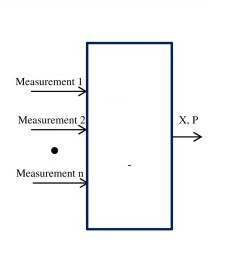
\includegraphics[scale=0.6]{img/sfaschema}
	\caption{Schema SFA}
	\label{fig:sfa}
\end{figure}
\clearpage
SFA viene eseguito su di un hardware installato a bordo treno, e la sua esecuzione \`e volta a monitorare costantemente il moto del treno.\\*
Il ciclo di esecuzione di SFA \`e essenzialmente una continua iterazione di due distinte fasi logiche:
\begin{itemize}
	\item Acquisizione delle misure;
	\item Predizione della posizione del treno.
\end{itemize}
Le grandezze fisiche che dovranno essere misurate e fornite a SFA sono:
\begin{itemize}
	\item Vettore accelerazione;
	\item Vettore velocit\`a angolare;
	\item Coordinate geografiche;
	\item Velocit\`a lineare (scalare).
\end{itemize}
In quest'applicazione, SFA utilizza tali informazioni in combinazione con un'apposita digitalizzazione della traccia tramviaria su cui si trova il treno monitorato.\cite{sfaimugps}\cite{sfaimuodo}\cite{sfaimuodogps} \\* Queste informazioni si suppongono note a priori ed accedibili tramite un \emph{database} caricato in memoria centrale. \cite{sqlite3}
\section{Sistemi Costituenti}
Il sottosistema di posizionamento si compone dei moduli, o \emph{Constituent Systems} (CS), descritti nel seguito di questa sezione.
\subsection{Sensor Set}
Il \emph{Sensor Set} \`e un insieme di sensori atti a campionare le misure richieste da SFA. Esso si compone a sua volta dei seguenti moduli:
\begin{itemize}
	\item \emph{Inertial Measurement Unit} (IMU):\\*
		Sensore inerziale incaricato di campionare e trasmettere a SFA i vettori \texttt{accelerazione} ($\mathbf{a}$) e \texttt{velocit\`a angolare} ($\mathbf{v_{ang}}$). Le misure di IMU sono prese rispetto alla Terra e sono espresse in unit\`a stabilite dallo standard internazionale (SI):
		$$
		\mathbf{a}\;\left[\frac{m}{s^2}\right]\;\;\;\;\mathbf{v_{ang}}\;\left[ \frac{rad}{s} \right]
		$$
		IMU \`e il sensore principale su cui si basa SFA nel predire la posizione del treno. Date le caratteristiche intrinseche del particolare SFA utilizzato, ossia un \emph{Filtro di Kalman}, il sistema funziona anche senza i rimanenti sensori. Si osserverebbe tuttavia un calo delle performance in termini di errore commesso sulla stima della posizione del treno. \cite{partialmeas} \cite{gpsdarkarea}
		\begin{figure}[h]
			\centering
			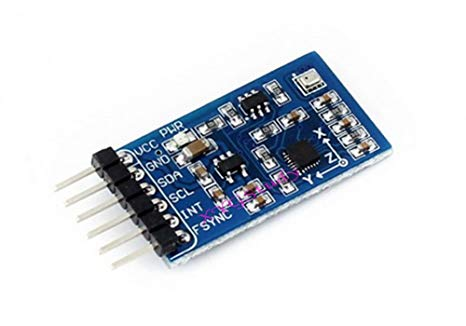
\includegraphics[scale=0.5]{img/imu}
			\caption{\emph{Inertial Measurment Unit}}
			\label{fig:imu}
		\end{figure}
		\item Odometro:\\*
		Unit\`a incaricata di fornire a SFA i valori di velocit\`a lineare del treno, espressi in $\frac{m}{s}$.
		\item GPS:
		\\*Unit\`a che fornisce a SFA le misure di posizione del treno.\\*
Le misure di GPS sono riportate in formato standard come tripla di coordinate \texttt{(latitudine, longitudine, altitudine)}, rispettivamente espresse in gradi \texttt{N-S}, in gradi \texttt{E-O} e in \texttt{metri} sul livello del mare.
\begin{figure}[h]
	\centering
	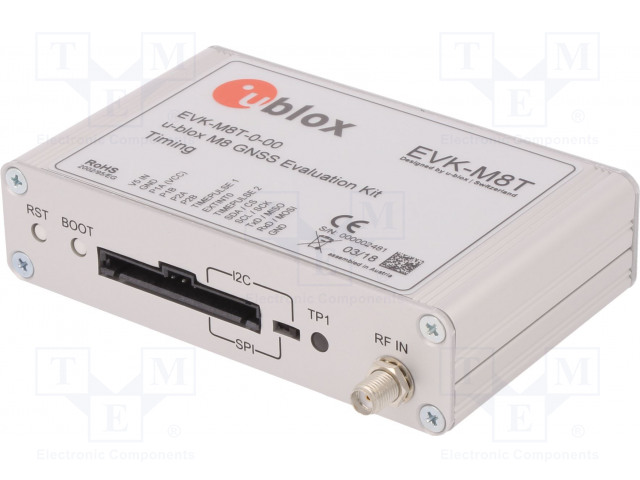
\includegraphics[scale=0.3]{img/gpsublox}
	\caption{Ricevitore \texttt{GPS ublox EVK-M8T}}
	\label{fig:gpsublox}
\end{figure}
\end{itemize}
\subsection{Piattaforma di elaborazione dati}
La piattaforma di elaborazione dati \`e l'hardware sul quale viene eseguito SFA.
Consiste di una scheda \texttt{Nvidia TX-Jetson} collegata al \emph{Sensor Set}.\\*
Da quest'ultimo essa riceve le misure da processare tramite SFA.
\begin{figure}[h]
		\centering
		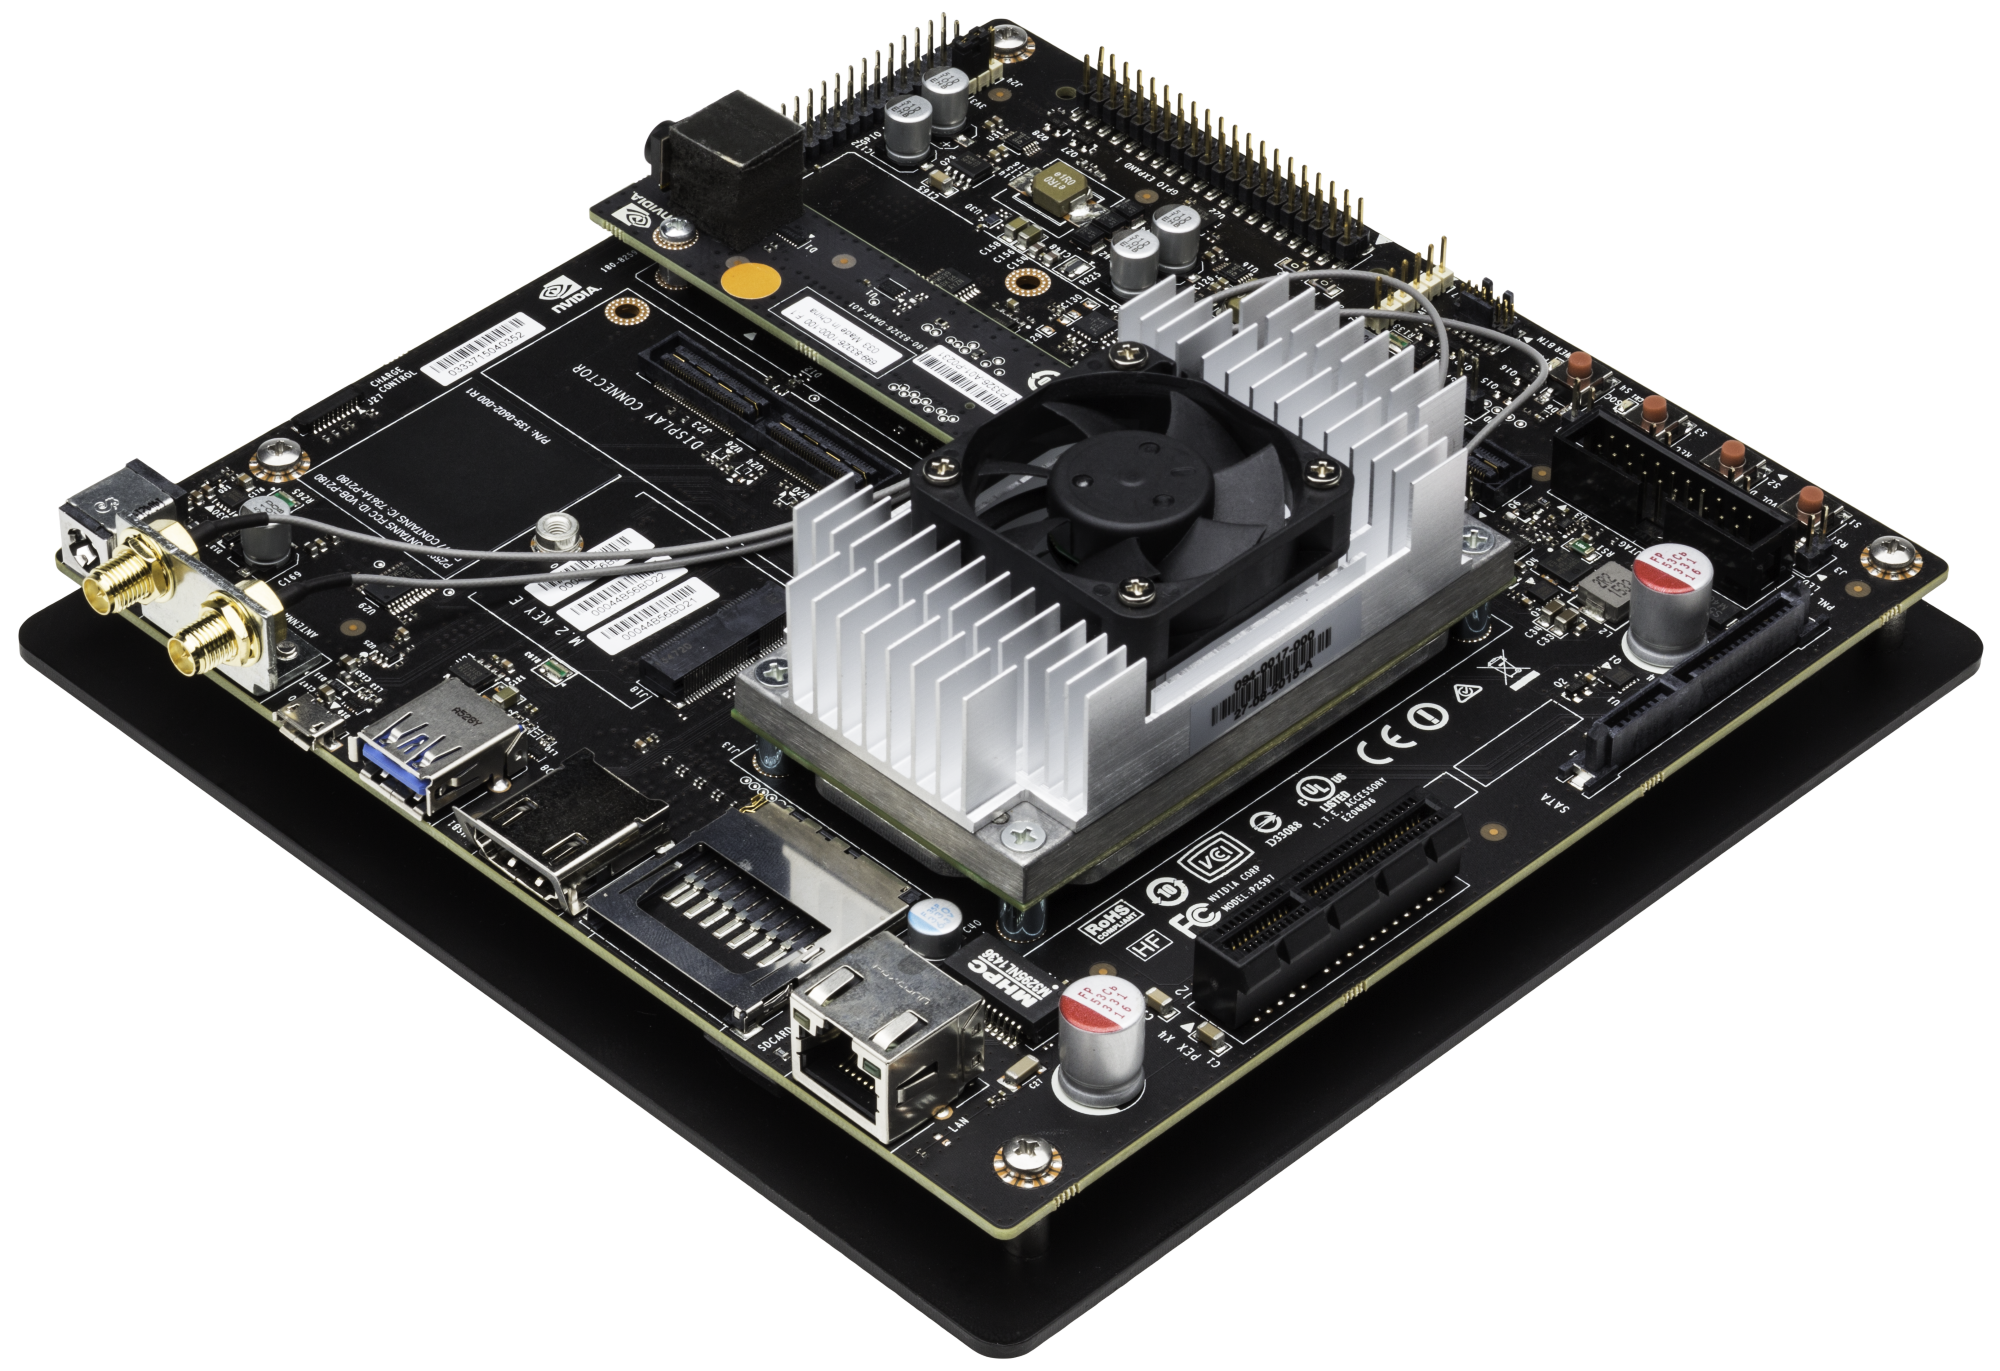
\includegraphics[width=0.7\linewidth]{img/nvidia}
		\caption{\texttt{Nvidia TX-Jetson}}
		\label{fig:nvidia}
\end{figure}
\texttt{Nvidia TX-Jetson} \`e un'architettura specifica per sistemi \emph{embedded}. Essa \`e ottimizzata per i calcoli computazionalmente onerosi tipici delle applicazioni di intelligenza artificiale.\cite{nvidia}\\*
\begin{table}[h]
\begin{tabular}{|p{3cm}|p{8cm}|}
	\hline 
	\textbf{GPU} & 256-core NVIDIA Pascal\\ 
	\hline 
	\textbf{CPU} & Dual-Core NVIDIA Denver 2 64-Bit CPU Quad-Core ARM Cortex-A57 MPCore \\ 
	\hline 
	\textbf{Memoria} & 8GB 128-bit LPDDR4 Memory \\ 
	\hline 
	\textbf{Storage} & 32GB eMMC 5.1 \\ 
	\hline 
	\textbf{Alimentazione} & 7.5W / 15W \\ 
	\hline 
\end{tabular}
\caption{Specifiche Tecniche \texttt{NVidia TX-Jetson}}
\label{tab:nvidia}
\end{table}
\subsection{On Board Control Unit}
L'\emph{On Board Control Unit} (OBCU) \`e il computer di bordo del treno. Esso non svolge alcun ruolo attivo nel sistema di posizionamento, tuttavia la progressiva chilometrica, stimata da SFA, dovr\'a essere trasmessa a OBCU al fine di poter utilizzare questa informazione all'interno del sistema di \emph{interlocking} della traccia.
	\section{Specifica delle Interfacce}
	\subsection{Relied Upon Interfaces}
	Le interfacce sono definite come punti di interazione, tra un CS e l'ambiente oppure tra un CS e un altro.\\*
	In questa sezione si evidenziano le principali interfacce del sistema, alle quali si osservano le interazioni fondamentali che avvengono al suo interno.\\*
	Tali interfacce prendono il nome di \emph{Relied Upon Interfaces} (RUI). Le RUI si dividono in:
	\begin{itemize}
		\item \emph{Relied Upon Physical Interfaces} (RUPI), in cui l'interazione avviene tramite osservazione diretta di una grandezza fisica;
		\item \emph{Relied Upon Message Interfaces} (RUMI), dove l'interazione \`e rappresentata da uno scambio di messaggi a livello \emph{cyber}.
	\end{itemize}
	La specifica delle RUI \`e di particolare importanza poich\'e qualunque struttura del sistema, responsabile del comportamento osservato, pu\'o essere ridotta alla specifica delle interfacce del sistema. \cite{interfacespec}\\*  
	Il CPS interagisce con l'ambiente attraverso le RUPI del \emph{Sensor Set}, ossia gli strumenti di misura che esso integra. Queste interfacce acquisiscono, a diverse frequenze, i dati sul moto del treno che verranno elaborati da SFA. Una descrizione sintetica delle RUPI del sistema \`e mostrata in tabella \ref{tab:rupi}.\\*
	\begin{table}[h]
	\centering
	\begin{tabular}{|c|c|c|}
		\hline 
		\textbf{RUPI} & \textbf{Grandezza Campionata}  & \textbf{Parti interagenti} \\ 
		\hline 
		Accelerometro & Accelerazione & Ambiente - IMU \\ 
		\hline 
		Giroscopio & Velocit\`a angolare & Ambiente - IMU  \\ 
		\hline 
		Radar & Velocit\`a lineare & Ambiente - Odometro \\ 
		\hline 
		Ricevitore GPS & Coordinate geografiche& Ambiente - GPS \\ 
		\hline 
	\end{tabular}
	\caption{Specifica delle RUPI del sistema}
	\label{tab:rupi}
	\end{table}\clearpage
	Per quanto concerne le RUMI, se ne osservano di due tipi:
	\begin{itemize}
		\item Tre bus dati, che collegano il \emph{Sensor Set} alla scheda \texttt{Nvidia TX-Jetson}. Su ciascuno di essi, \emph{Sensor Set} invia rispettivamente messaggi contenenti i dati campionati da IMU, Odometro e GPS.
		\item Interfaccia LTE. Essa permette di realizzare una \emph{rete wireless ad hoc} fra la scheda e OBCU.\\*
		All'interno di tale rete vengono instradati datagrammi \texttt{IP} contenenti le informazioni sulla progressiva chilometrica stimata da SFA, ed eventualmente messaggi di \emph{acknowledgment} di OBCU verso la scheda.
		\begin{figure}[h]
			\centering
			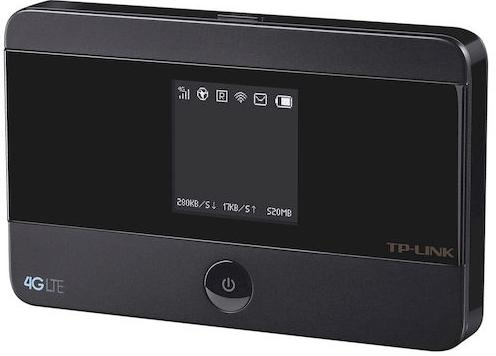
\includegraphics[scale=0.40]{img/lte}
			\caption{Modem \texttt{TP-LINK M7350 LTE-4G}}
			\label{fig:lte}
		\end{figure}
	\end{itemize}
	\begin{figure}[h]
		\centering
		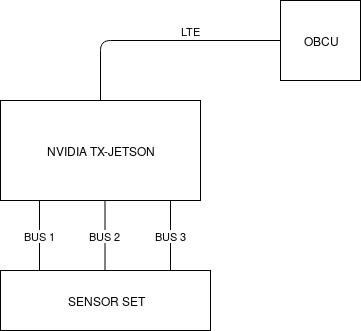
\includegraphics[width=0.7\linewidth]{img/TrainDiagram}
		\caption{Architettura hardware del sottosistema di posizionamento}
		\label{fig:tdiagram}
	\end{figure}
		\begin{table}[h]
		\centering
		\begin{tabular}{|c|c|c|}
			\hline 
			\textbf{RUMI} & \textbf{Informazione trasmessa}  & \textbf{Parti interagenti} \\ 
			\hline 
			Bus Dati 1 & Accelerazione, Velocit\`a angolare & Sensor Set - \texttt{NVidia TX-Jetson} \\ 
			\hline 
			Bus Dati 2 & Velocit\`a lineare & Sensor Set - \texttt{NVidia TX-Jetson} \\ 
			\hline 
			Bus Dati 3 & Coordinate geografiche & Sensor Set - \texttt{NVidia TX-Jetson} \\ 
			\hline 
			LTE & Posizione del treno & \texttt{NVidia TX-Jetson} - OBCU \\ 
			\hline 
		\end{tabular}
		\caption{Specifica delle RUMI del sistema}
		\label{tab:rumi}
	\end{table}
\newpage
	\section{Interazioni}
	In questa sezione si descrivono le interazioni osservabili alle interfacce sopra descritte. Queste possono essere in prima istanza categorizzate a discrezione della fase di SFA in cui esse avvengono.\\*
	Si distinguono pertanto le interazioni riguardanti l'acquisizione dei dati in ingresso a SFA, e le interazioni riguardanti l'acquisizione da parte di OBCU della posizione del treno.
	\subsection{Acquisizione dei dati}
	L'acquisizione dei dati si divide in due differenti interazioni: la prima, con l'ambiente, avviene alle RUPI del \emph{Sensor Set}, mentre la seconda avviene alle RUMI bus dati che collegano il \emph{Sensor Set} alla piattaforma di elaborazione dati.\\*
	I moduli che compongono il \emph{Sensor Set} campionano ad una data frequenza le grandezze fisiche che descrivono il moto del treno. Ciascun campionamento fisico \`e seguito dall'invio dei valori letti alla piattaforma di elaborazione dati. I moduli del \emph{Sensor Set} sono tra di loro indipendenti.\\* 
	In figura \ref{fig:seqdiag} viene riportato un \emph{sequence diagram} rappresentante una possibile sequenza di campionamento e invio dei dati.\newpage	\begin{figure}[h]
		\centering
		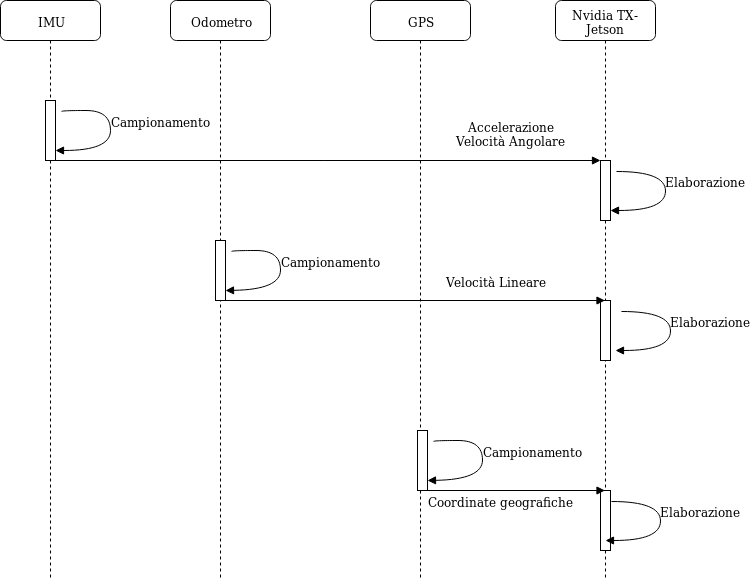
\includegraphics[width=0.7\linewidth]{img/seqdiag}
		\caption{Sequenza di acquisizione dati}
		\label{fig:seqdiag}
	\end{figure}
	Questa tipologia di interazione \`e detta \emph{time-triggered}, in quanto \`e determinata unicamente dallo scorrere del tempo. \cite{timetriggered}
	\subsection{Trasmissione della posizione}
	La piattaforma di elaborazione dati esegue SFA durante l'intero moto del treno. Le misure fornite dai sensori vengono elaborate al fine di aggiornare continuamente la stima della posizione del treno.\\*
	Ogniqualvolta venga completato un aggiornamento di SFA, si osserva un'interazione all'interfaccia LTE. Tale interazione consiste nell'invio di un messaggio contenente la posizione del treno, dalla piattaforma di elaborazione dati verso OBCU, e nella trasmissione di un messaggio di \emph{acknowledgment} nel senso opposto.\\*
	La tipologia di scambio dei messaggi esposta \`e detta \emph{event-triggered} \cite{evttimetriggered} in quanto le tempistiche di interazione non sono note a priori, ma dipendono dal tempo computazionale impiegato da SFA nell'aggiornare la propria stima della posizione.\\*
	LTE \`e a tutti gli effetti una regolare interfaccia di rete. Il messaggio trasmesso \`e contenuto nel \emph{payload} di un datagramma \texttt{UDP}; in accordo al modello di rete \texttt{ISO-OSI}. \cite{libroreti}
	\begin{figure}[h]
		\centering
		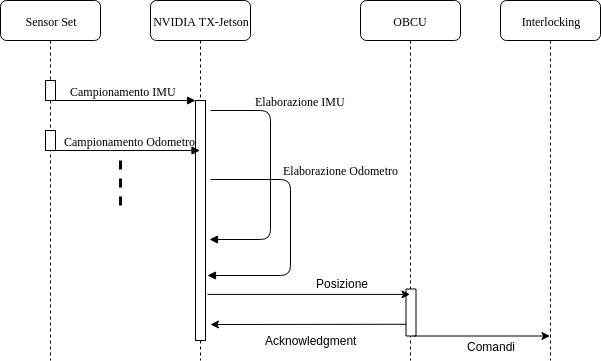
\includegraphics[width=0.7\linewidth]{img/seqdiag2}
		\caption{Sequenza di trasmissione della posizione}
		\label{fig:seqdiag2}
	\end{figure}
	\subsection{Interazioni con eventuali operatori umani}
	La filosofia del sistema oggetto della Tesi include la minimizzazione di interventi da parte di operatori umani.\\*
	A questi viene lasciato il compito di predisporre le informazioni geografiche della traccia nel database, e di segnalare l'avvio al sistema.\\*
	Il processo che esegue SFA \`e in effetti un \emph{demone} che si avvia contestualmente all'accensione della piattaforma.\\*
	Viene infine predisposta un interfaccia \texttt{SSH} per accedere da remoto alla piattaforma a scopi di \emph{deployment} o di \emph{monitoring online} attraverso la lettura dei file di \emph{log}.